\subsection{Primary Stakeholders}
    \indent\indent \textit{Students} - Students, particularly those who have recently become independent, are the target audience for our app as this demographic contributes disproportionately to food waste in the UK. Entering into a new environment with increased responsibilities results in many students becoming neglectful of less present problems such as the food expiring in their fridge. The WRAP UK Household Food Management Survey 2024\cite{waringPleaseUseThis} supports this assertion, attributing increased household food waste to traits highly prevalent among students\cite{gamboa-delgadoFactorsAssociatedFood2024, landryBarriersCollegeStudent2024} including competency and living circumstances – 49\% of “those who judge themselves weaker at judging and buying the right amount [of food]” and 31\% of “those who agree to feeling under time pressure” were categorized as high food wasters, clearly exceeding the population mean of 27\%. Through surveying students from several universities\cite{STUDENT SURVEY, FRESHER SURVEY} we uncovered that the majority of students “sometimes” disposed of food items due to them being out of date, with this being especially pervasive among first year students. The primary reasons cited for this wastage were “I forgot it was there” and “I was unable to use all of the ingredient”. From this response we have decided to tailor our app to include notifications to remind students about food expiry dates as well as a meal recommendation feature for leftovers, with the desired outcome being to reduce the responsibility for students to check their food and plan their meals so that the amount of expired food items students dispose of weekly decreases.\\
    \par
    \textit{Developers} – As developers we are the technical specialists responsible for designing, building and maintaining the app. Our role is to ensure that the app is both efficient and meets the users’ needs, particularly with regards to features such as date code scanning, expiry date notifications and meal recommendations for leftovers. We are therefore directly affected by the app in the forms of workload, technical challenges and app maintenance. Consequently, our goal is to produce a reliable, effective, secure app that achieves our goal of reducing the amount of unnecessary food waste produced by students and other demographics. \\
    \par
    \textit{Other Primary Stakeholders include:} Parents and Other Potential App Users
\subsection{Secondary Stakeholders}
    \indent\indent \textit{Supermarkets} – Supermarkets will be indirectly affected by our app since it is intended to empower consumers to better manage their food at home, reducing household waste that originates from supermarket purchases. This strengthens the supermarket’s sustainability profile and enhances their reputation for environmental responsibility. Our app would therefore aim to align with the major objectives of supermarkets\cite{WRAPSRETAILSURVEY} – being to strengthen their drive for environmental sustainability, enhance customer loyalty, and gain insights into post-purchase food management – while balancing potential impacts on sales volumes. Furthermore, future app iterations could potentially see users receiving expiry dates directly from the supermarket checkouts, deepening collaboration between the app and supermarket and so reinforcing customer loyalty towards both the app and supermarket.\\
    \par
    \textit{Local Councils} – In the long-term local councils will be indirectly affected by our app and so are considered secondary stakeholders. By reducing food waste among individual students, parents and other users, communities will consequently see a reduction in food waste. As of 2022 local authorities in the UK have been mandated to reduce food waste by prioritising household waste prevention through public behaviour change\cite{peacockLocalAuthorityCollected}, while also ensuring weekly separate food waste collections that divert unavoidable waste from landfill to recycling or energy recovery. Moreover, in March 2024 the UK Government announced a “new £295 million for councils to introduce weekly food waste collection”\cite{NewPS295mCouncils}, money local councils could reallocate to address other local issues (such as increased local public transport\cite{HowLocalTransport2024}) if they faced less pressure to reduce food waste. The desired outcome of our app towards local councils would be to alleviate the financial and political pressure created by high food waste among communities, allowing them to reduce money allocated to food waste and instead focus it towards other more pressing issues.\\
    \par
    \textit{Other Secondary Stakeholders Include:} Housemates, the Taxpayer
\subsection{Tertiary Stakeholders}
	\indent\indent \textit{Our Tertiary Stakeholders Include:} Environmental NGO’s and Sustainability Organisations (e.g. WRAP), Policy Makers\\
    \\

\begin{figure}[h!]
\centering
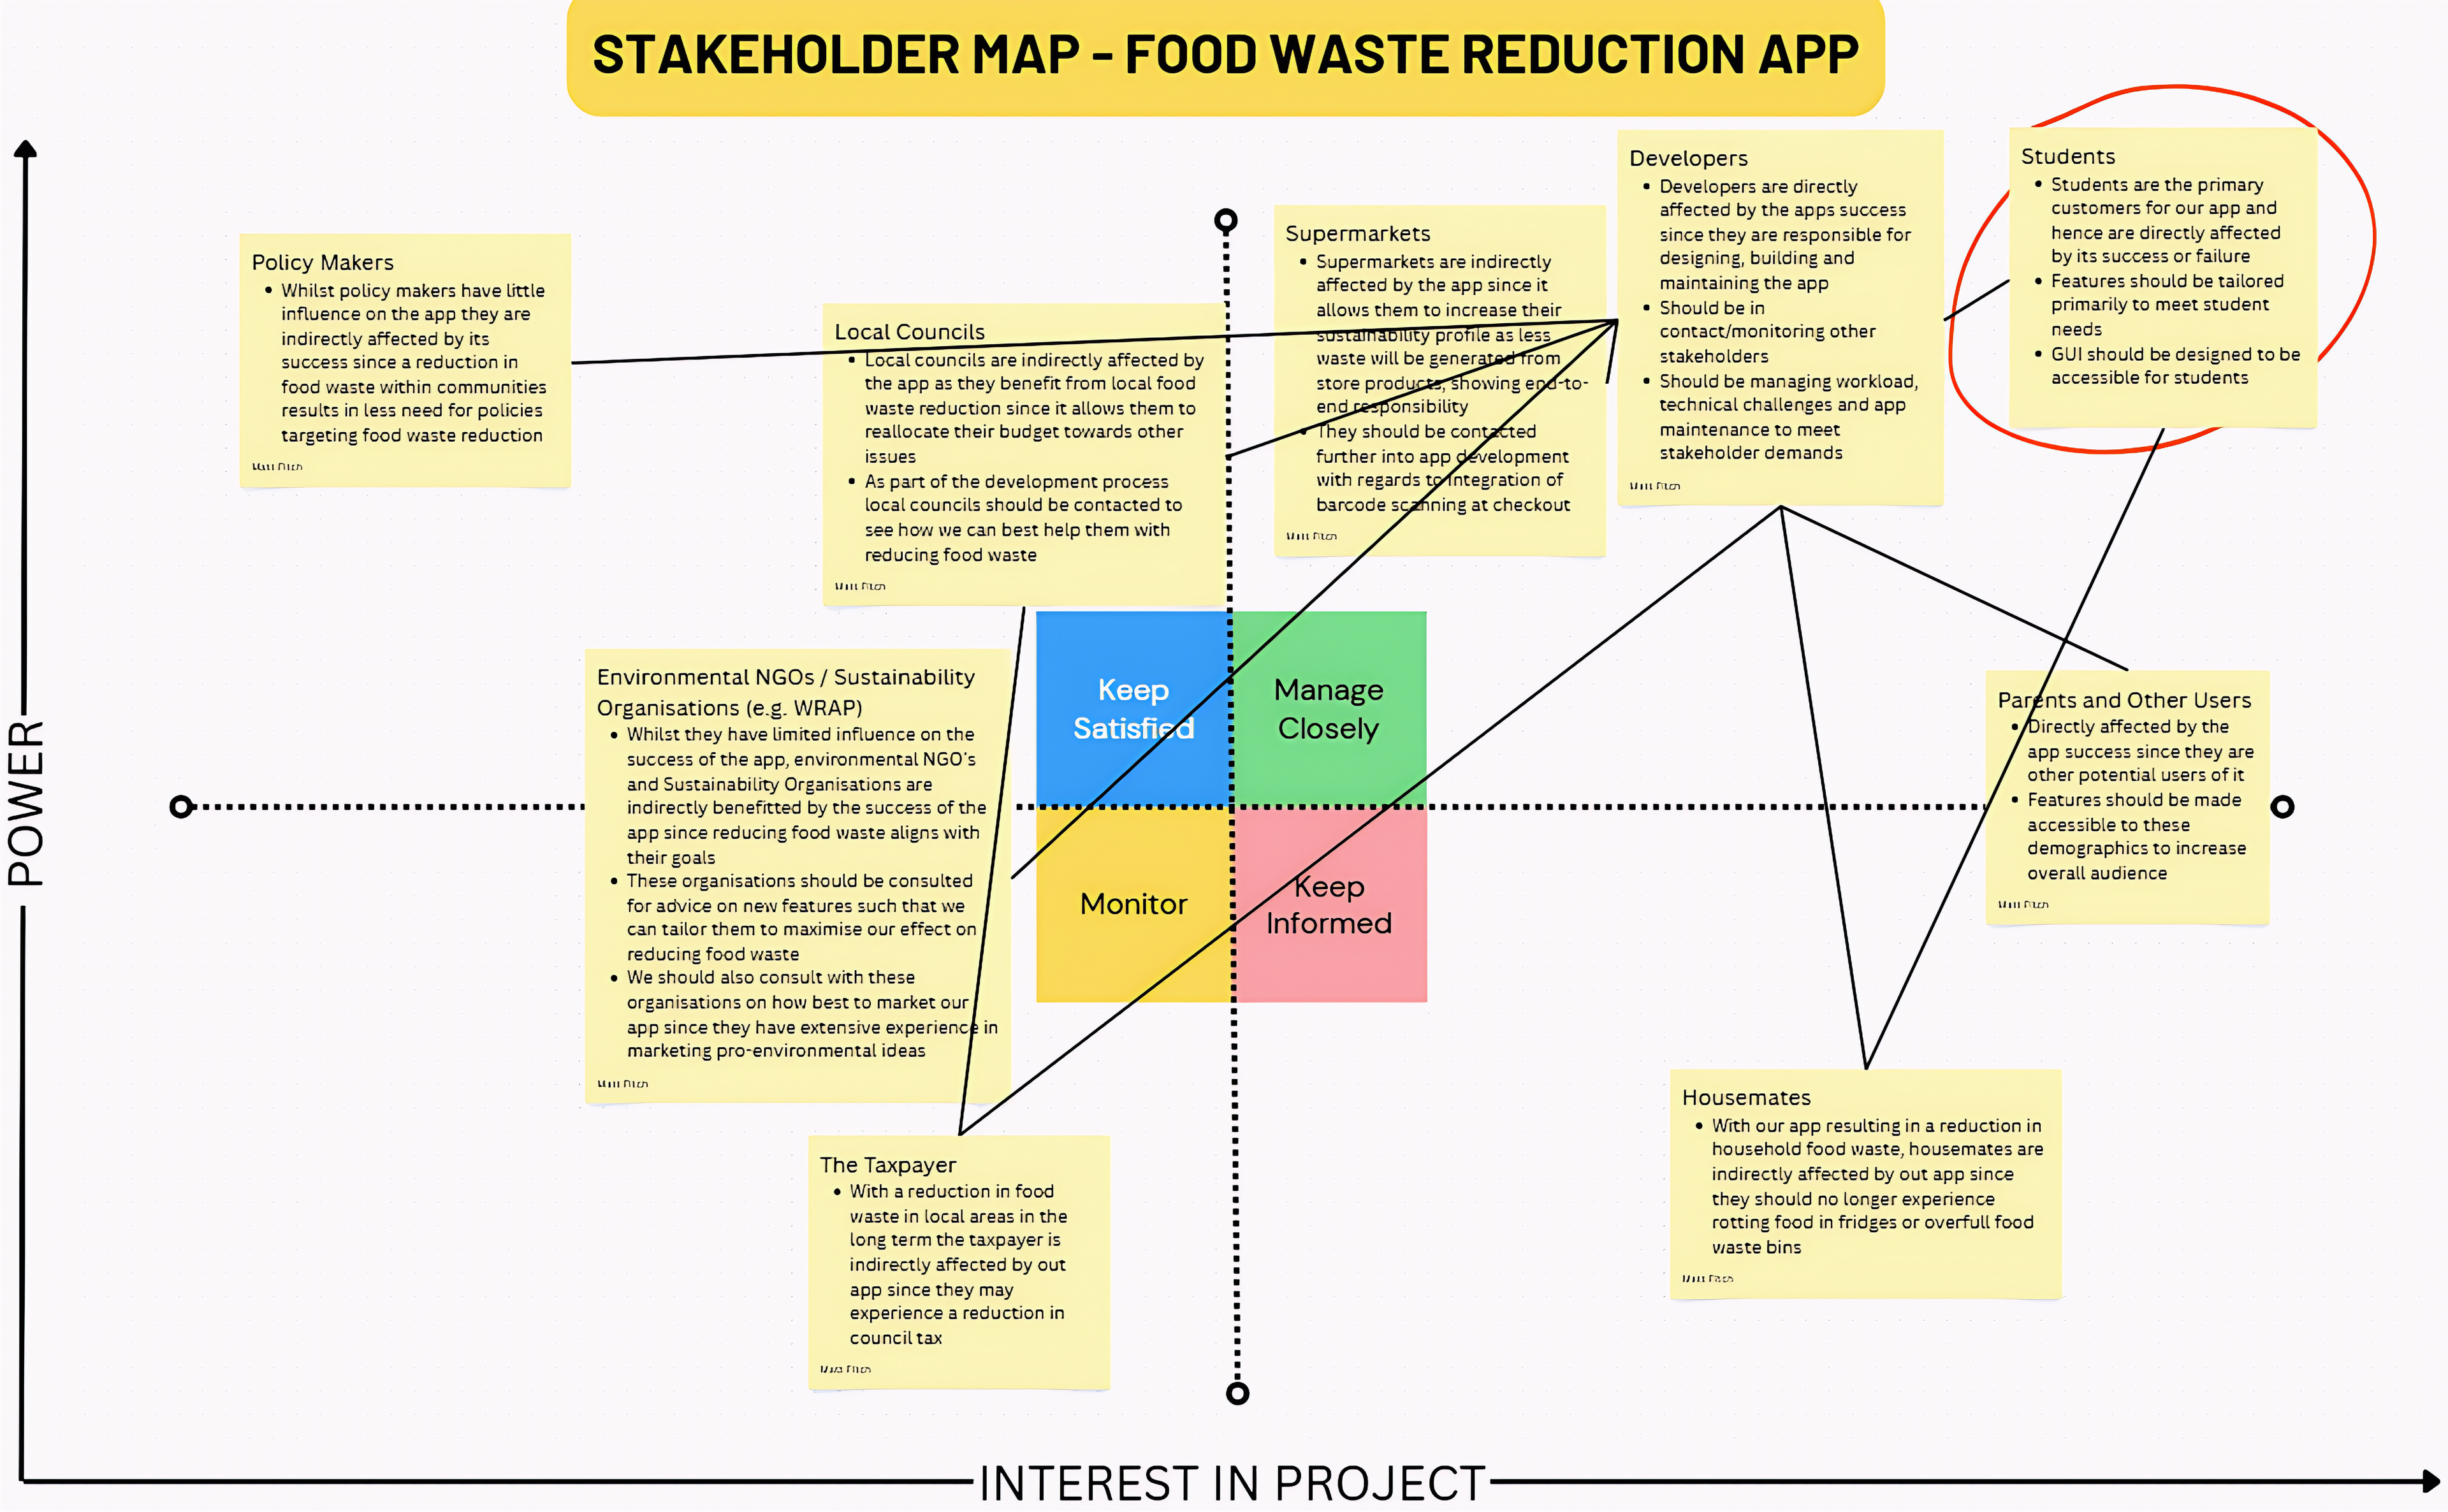
\includegraphics[width=1\linewidth]{Stakeholder Map - FWRA_imgupscaler.ai_General_4K.jpg}
\caption{\label{fig: Stakeholder Map}Stakeholder Map}
\end{figure}




